\documentclass[letterpaper,12pt]{article}
\usepackage{tabularx} % extra features for tabular environment
\usepackage{amsmath}  % improve math presentation
\usepackage{float}
\usepackage{pdfpages}

\usepackage{graphicx} % takes care of graphic including machinery
\graphicspath{ {./figures/} }
\usepackage[margin=1in,letterpaper]{geometry} % decreases margins
\usepackage{cite} % takes care of citations
\usepackage[final]{hyperref} % adds hyper links inside the generated pdf file
\hypersetup{
	colorlinks=true,       % false: boxed links; true: colored links
	linkcolor=blue,        % color of internal links
	citecolor=blue,        % color of links to bibliography
	filecolor=magenta,     % color of file links
	urlcolor =blue         
}




\begin{document}

\title{Experiment 3 Preliminary Work \protect\\ Transformers and MATLAB Workshop}
\author{Ahmet Akman 2442366 \protect\\}
\date{\today}
\maketitle
\tableofcontents
%\begin{abstract}
%abstract
%\end{abstract}

%\section{Introduction}
\section{Step 1}
The document entitled,  "Supplementary Notes on Transformers", is studied.
\section{Step 2}
The document entitled,  "Introduction to MATLAB", is studied.
\section{Step 3}
In this step the signal data given in ODTUClass are taken as reference. The signals can be represented as;
\[
v_1 = 7.5 sin(2\pi 100t) \\
\]\[ 
v_2 = 2.5 sin(2\pi 300t) \\
\]\[ 
v_3 = 1.5 sin(2\pi 500t)    
\] 
First the signals are plotted in same figure and given Figure 1.
\begin{figure}[H]
    \centering
    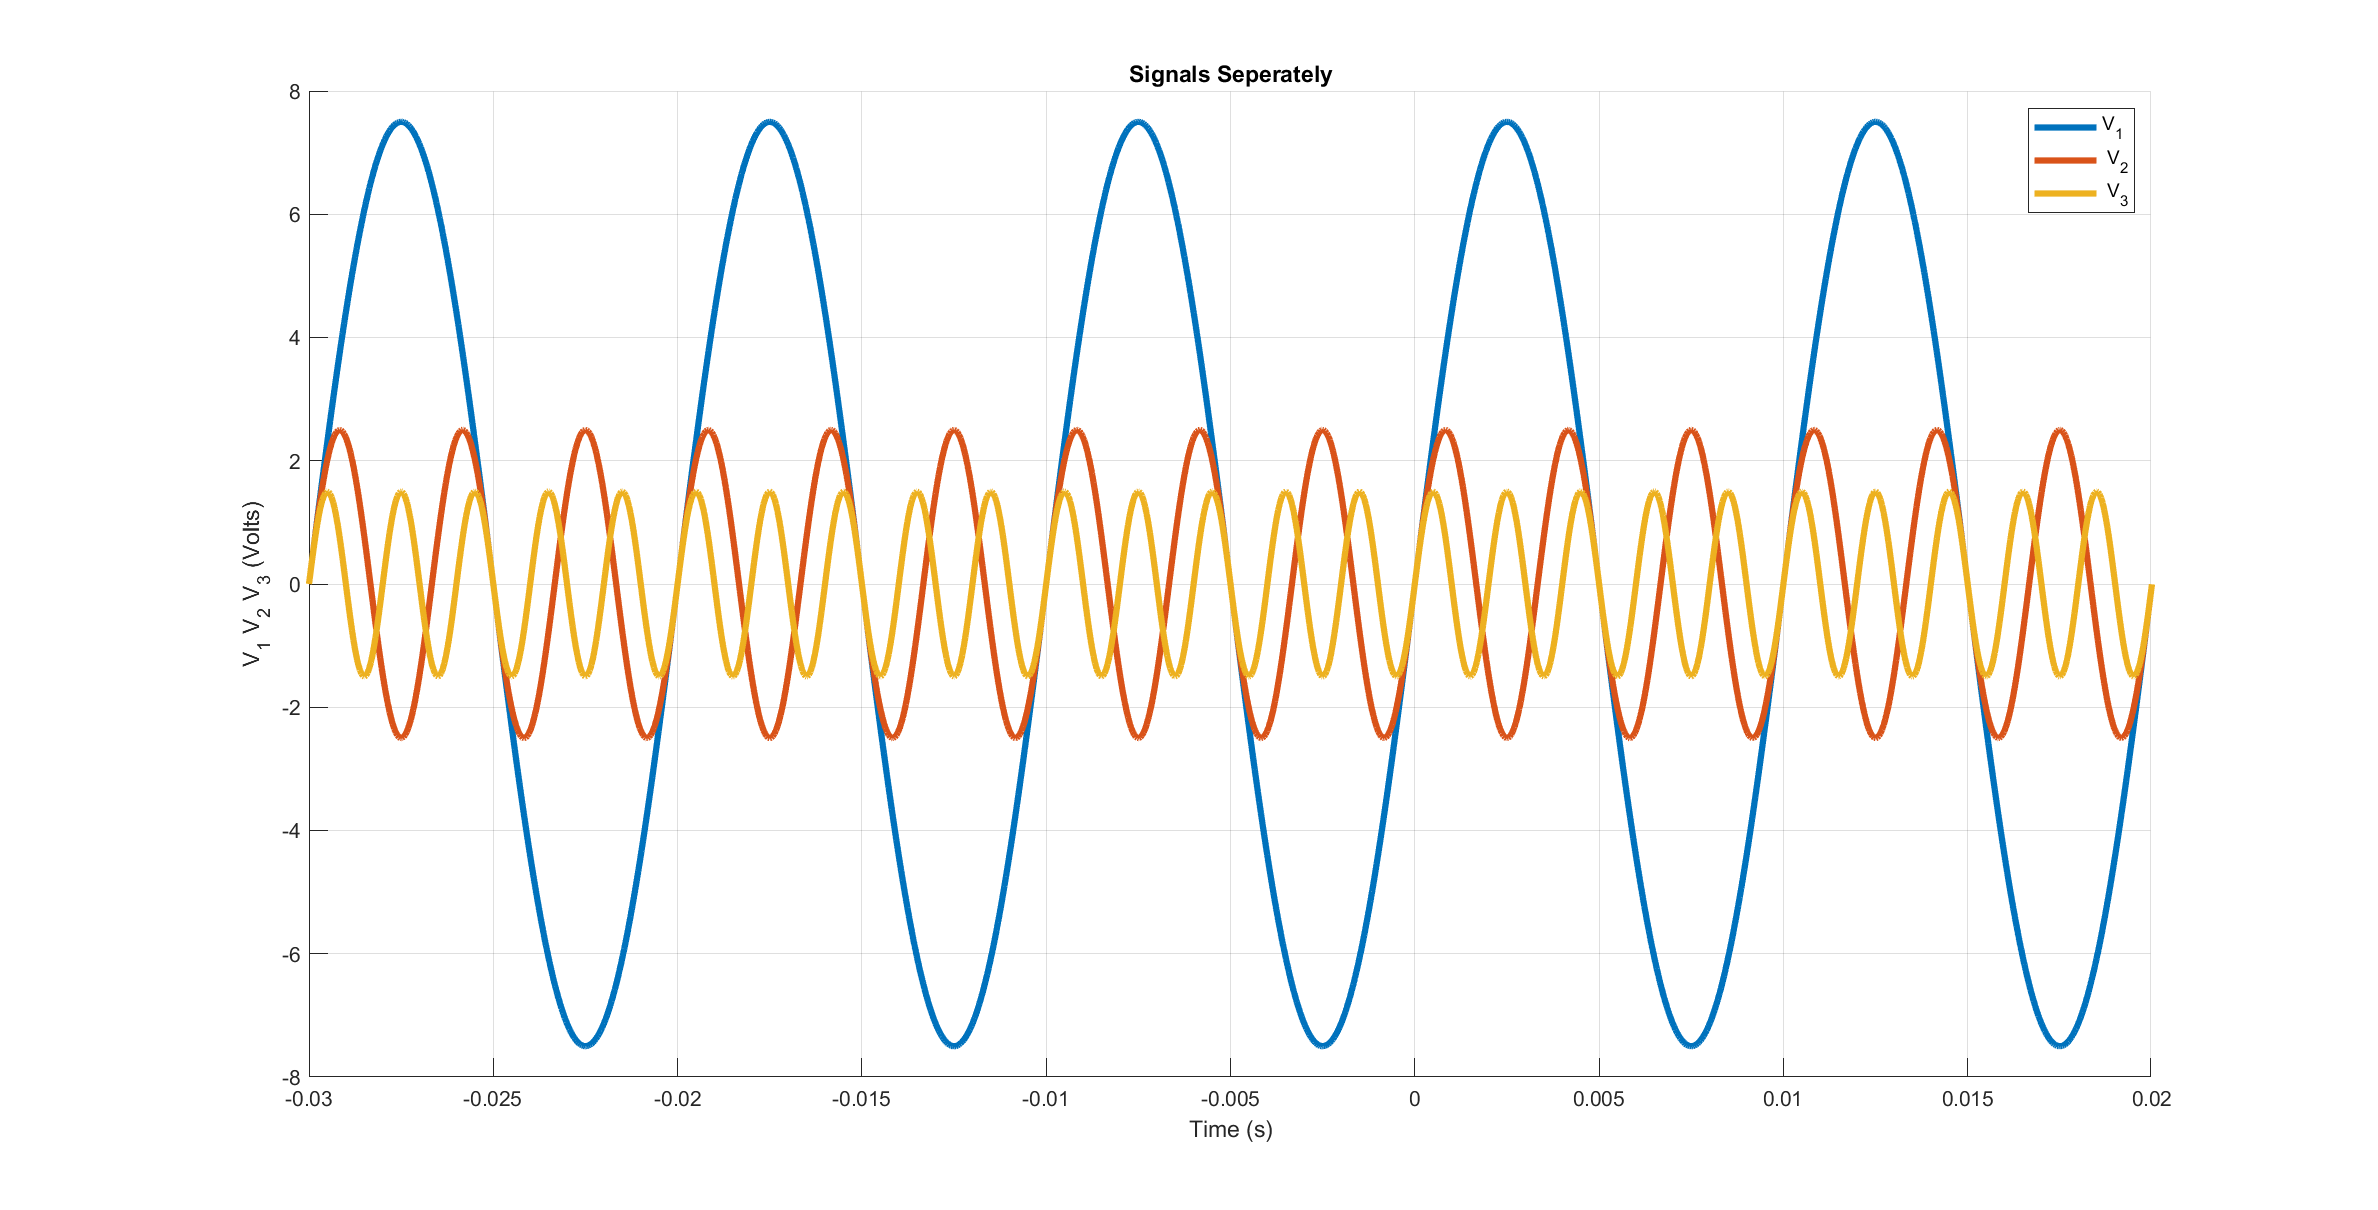
\includegraphics[width=1\textwidth]{3a.png}
    \caption{All three signals seperately}
\end{figure} 
Then the signals are plotted progressively. First only the v1 signal is plotted. Then the sum of v1 and v2 is plotted. Lastly, sum of all three signals is plotted. 
\begin{figure}[H]
    \centering
    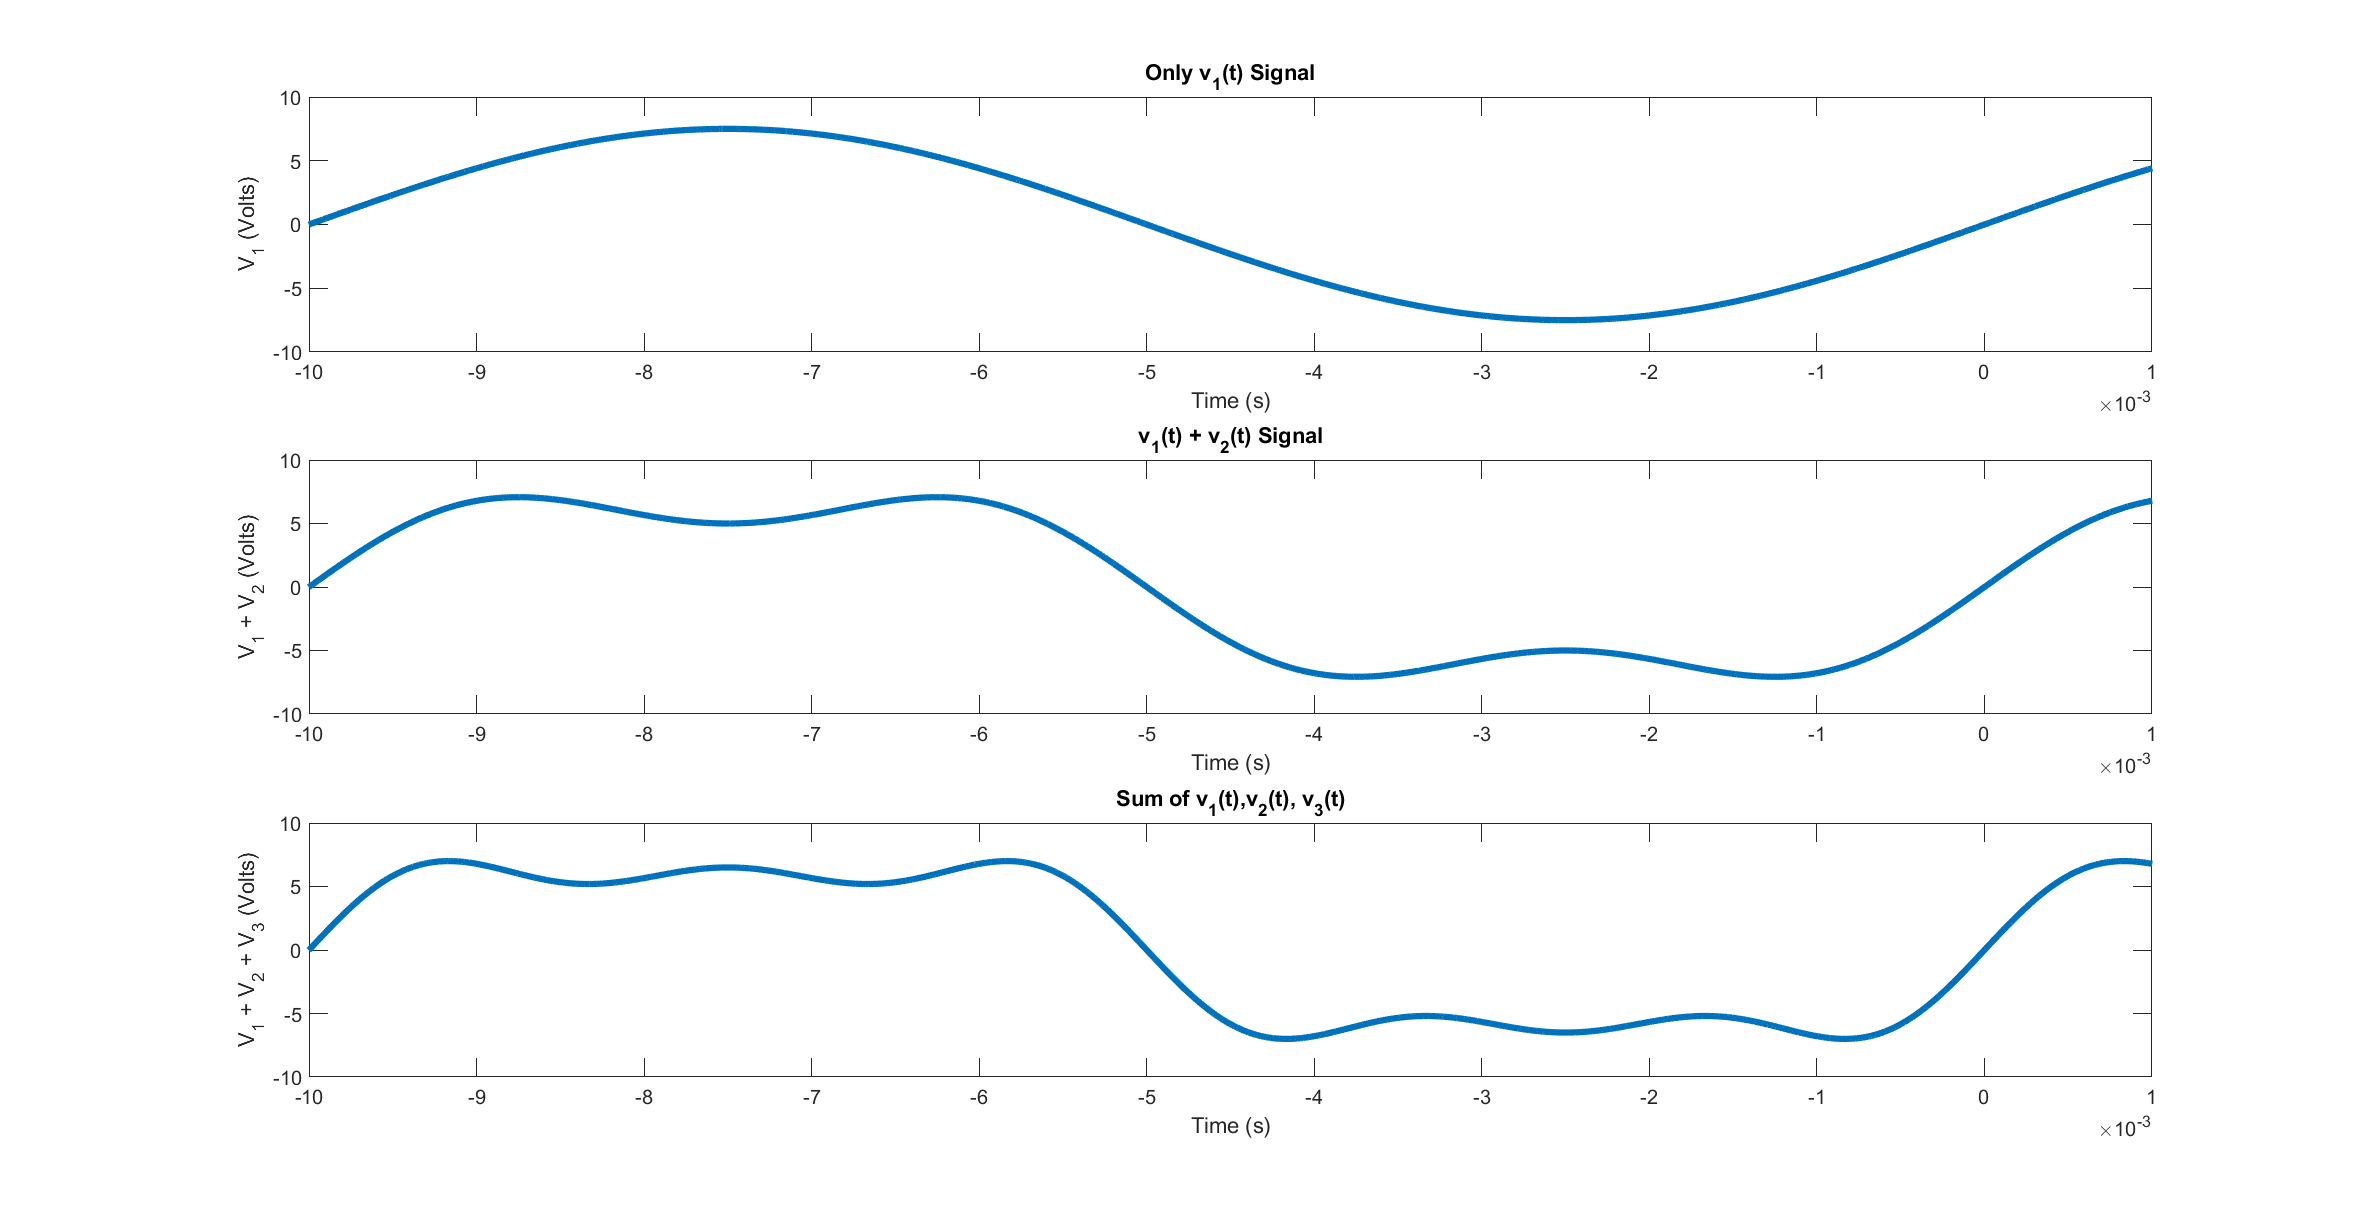
\includegraphics[width=1\textwidth]{3b.png}
    \caption{Progressive plot}
\end{figure} 
As a result it can be said that as the different sine waves sums it approaches a square wave. So it is understood that perfect square wave is a sum of infinite square sine wave.

\section{Conclusion}
In this preliminary work document. Necessary documents are studied. Then it is observed how one can represent a square wave as the sum of different sine waves.

\iffalse
\section*{Appendix A}
The results of the simulations are fetched from LTSpice and plotted in MATLAB in order to make the plots more readable and convenient.
\fi

\end{document}

%%%%%%%%%%%%%%%%%%%%%%   EXAMPLE TABLE   %%%%%%%%%%%%%%%%%%%%%%%%%%%%%%%%
\begin{table}[H]
\begin{center}
    \caption{Resistance reading by color code convention.}
    \vspace{2mm}
    \begin{tabular}{||c | c | c||} 
        \hline
        Color Order & Value & Tolerance \\ [0.5ex] 
        \hline\hline
        Brown / Black / Red / Gold & 1k\( \Omega \) & \( \% \) 5  \\ 
        \hline
        Yellow / Violet / Red / Gold & 4.7k\( \Omega \) & \( \% \) 5   \\
        \hline
        Brown / Grey / Orange / Gold & 18k\( \Omega \) & \( \% \) 5  \\ [1ex] 
        \hline
    \end{tabular}
\end{center}
\end{table}


%%%%%%%%%%%%%%%%%%%%%%   EXAMPLE IMAGE   %%%%%%%%%%%%%%%%%%%%%%%%%%%%%%%%
\begin{figure}[H]
\centering
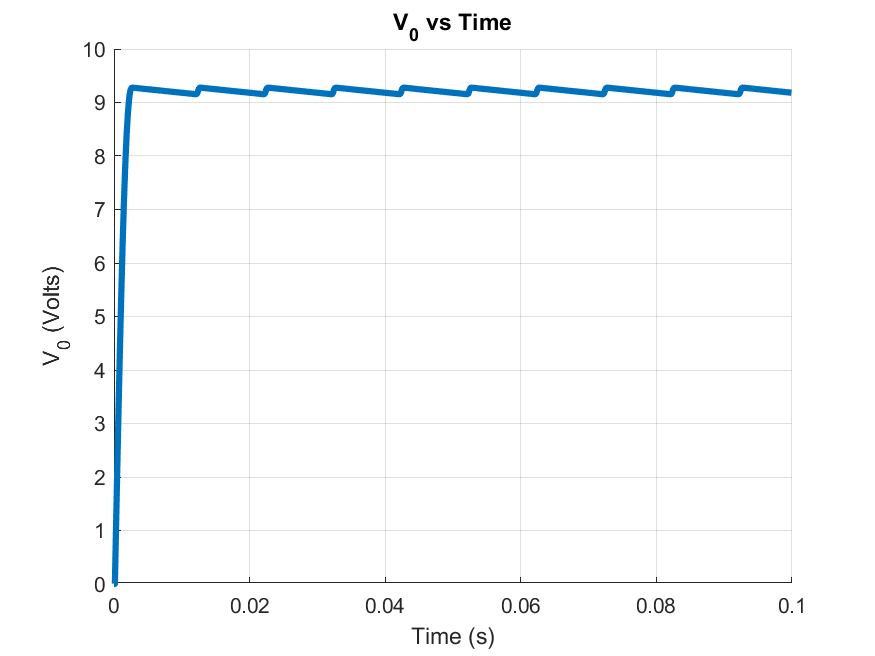
\includegraphics[width=1\textwidth]{5.png}
\caption{Circuit schematic for the step 5}
\end{figure} 

%%%%%%%%%%%%%%%%%%%%%%   EXAMPLE IMAGE FROM PDF   %%%%%%%%%%%%%%%%%%%%%%%%%%%%%%%%
\begin{figure}[H] \centering{
	\includegraphics[scale=0.25]{2a_plot.pdf}}
	\caption{Experiment 2}
\end{figure}
	